% https://arxiv.org/pdf/1312.6034v2.pdf - Deep Inside Convolutional Networks: Visualising Image Classification Models and Saliency Maps

% Gradient: Technik um größten Anstieg zu finden -> man nimmt also beim Trainieren den negativen Gradient: -Delta(->W) = [0.2 -1 ...] // GIbt an wie die Weights verändert werden sollten
% Numerische Approximation des Gradients: https://en.wikipedia.org/wiki/Numerical_differentiation
% Gradient Descent/ Full Backpropagation): mache es für alle Trainingsamples und nehme den durchschnitt
% Stochasitic Gradient Descent: Nehm ein paar und nehme den Durchschnitt
% Backpropagation: Determine how one trainign example want to change the weights and biases

\section{Deep Dream Algorithm}
\label{sec:how}

This section introduces the visual and mathematical aspects of the \emph{Deep Dream} algorithm.

\subsection{TODO: Visual Aspects}
\label{sec:visual-aspects}
Deep Dreaming requires a pretrained image recognition neural network and a source image one wishes to modify.
The source image can be any arbitrary image.
Figure \ref{fig:neuronreact} portrays a small section of an abstract unspecified neural network.
The small embedded images in the neurons are examples of features that they learned.
The combination of all these small features leads to the conclusion of the network.

For the dream one can choose an individual or a set of neurons which should be more activated.
This is done by modifying the image in such a way that the learned features of  neurons are more present.

An example of this is given in figure \ref{fig:applieddream}.
Here the neuron on the top of figure \ref{fig:neuronreact} was chosen.
Hence the image was modified such that the learned features dominates the visual appearance of the image.

Since it would be close to impossible to find the right combination of neurons to draw a specific object, there is the possibility of using a \textit{Guided Dream}.
The concrete inner workings of the \textit{Guided Dream} are explained in section \ref{guided-dreaming}.
For a \textit{Guided Dream} there is a second image involved, which will be referred to as \textit{Guide Image}.
This image is processed by the network and the activations are tracked to modify the source image so that it contains similar features as the guide.

As a relatable real life example imagine looking into the clouds.
Some of them remind you of familiar objects and your mind transforms them into more like those.
You can think of \emph{Deep Dream} working in a similar manner.
It is much more thorough in the amount of features it detects.
The differentiation to a \emph{Guided Dream} would then trying to project specific objects into the clouds.

\begin{figure}[H]
	\centering
	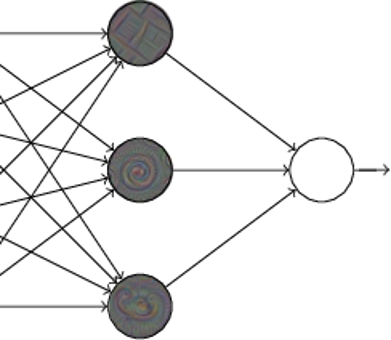
\includegraphics[width=0.5\linewidth]{img/neurons-reaction.png}
	\caption{TODO: "CAT" entfernen A small section of an abstract unspecified neural network. The neurons contain artificial features.\cite{nielsen2015neural}.}
	\label{fig:neuronreact}
\end{figure}

\begin{figure}[H]
	\centering
	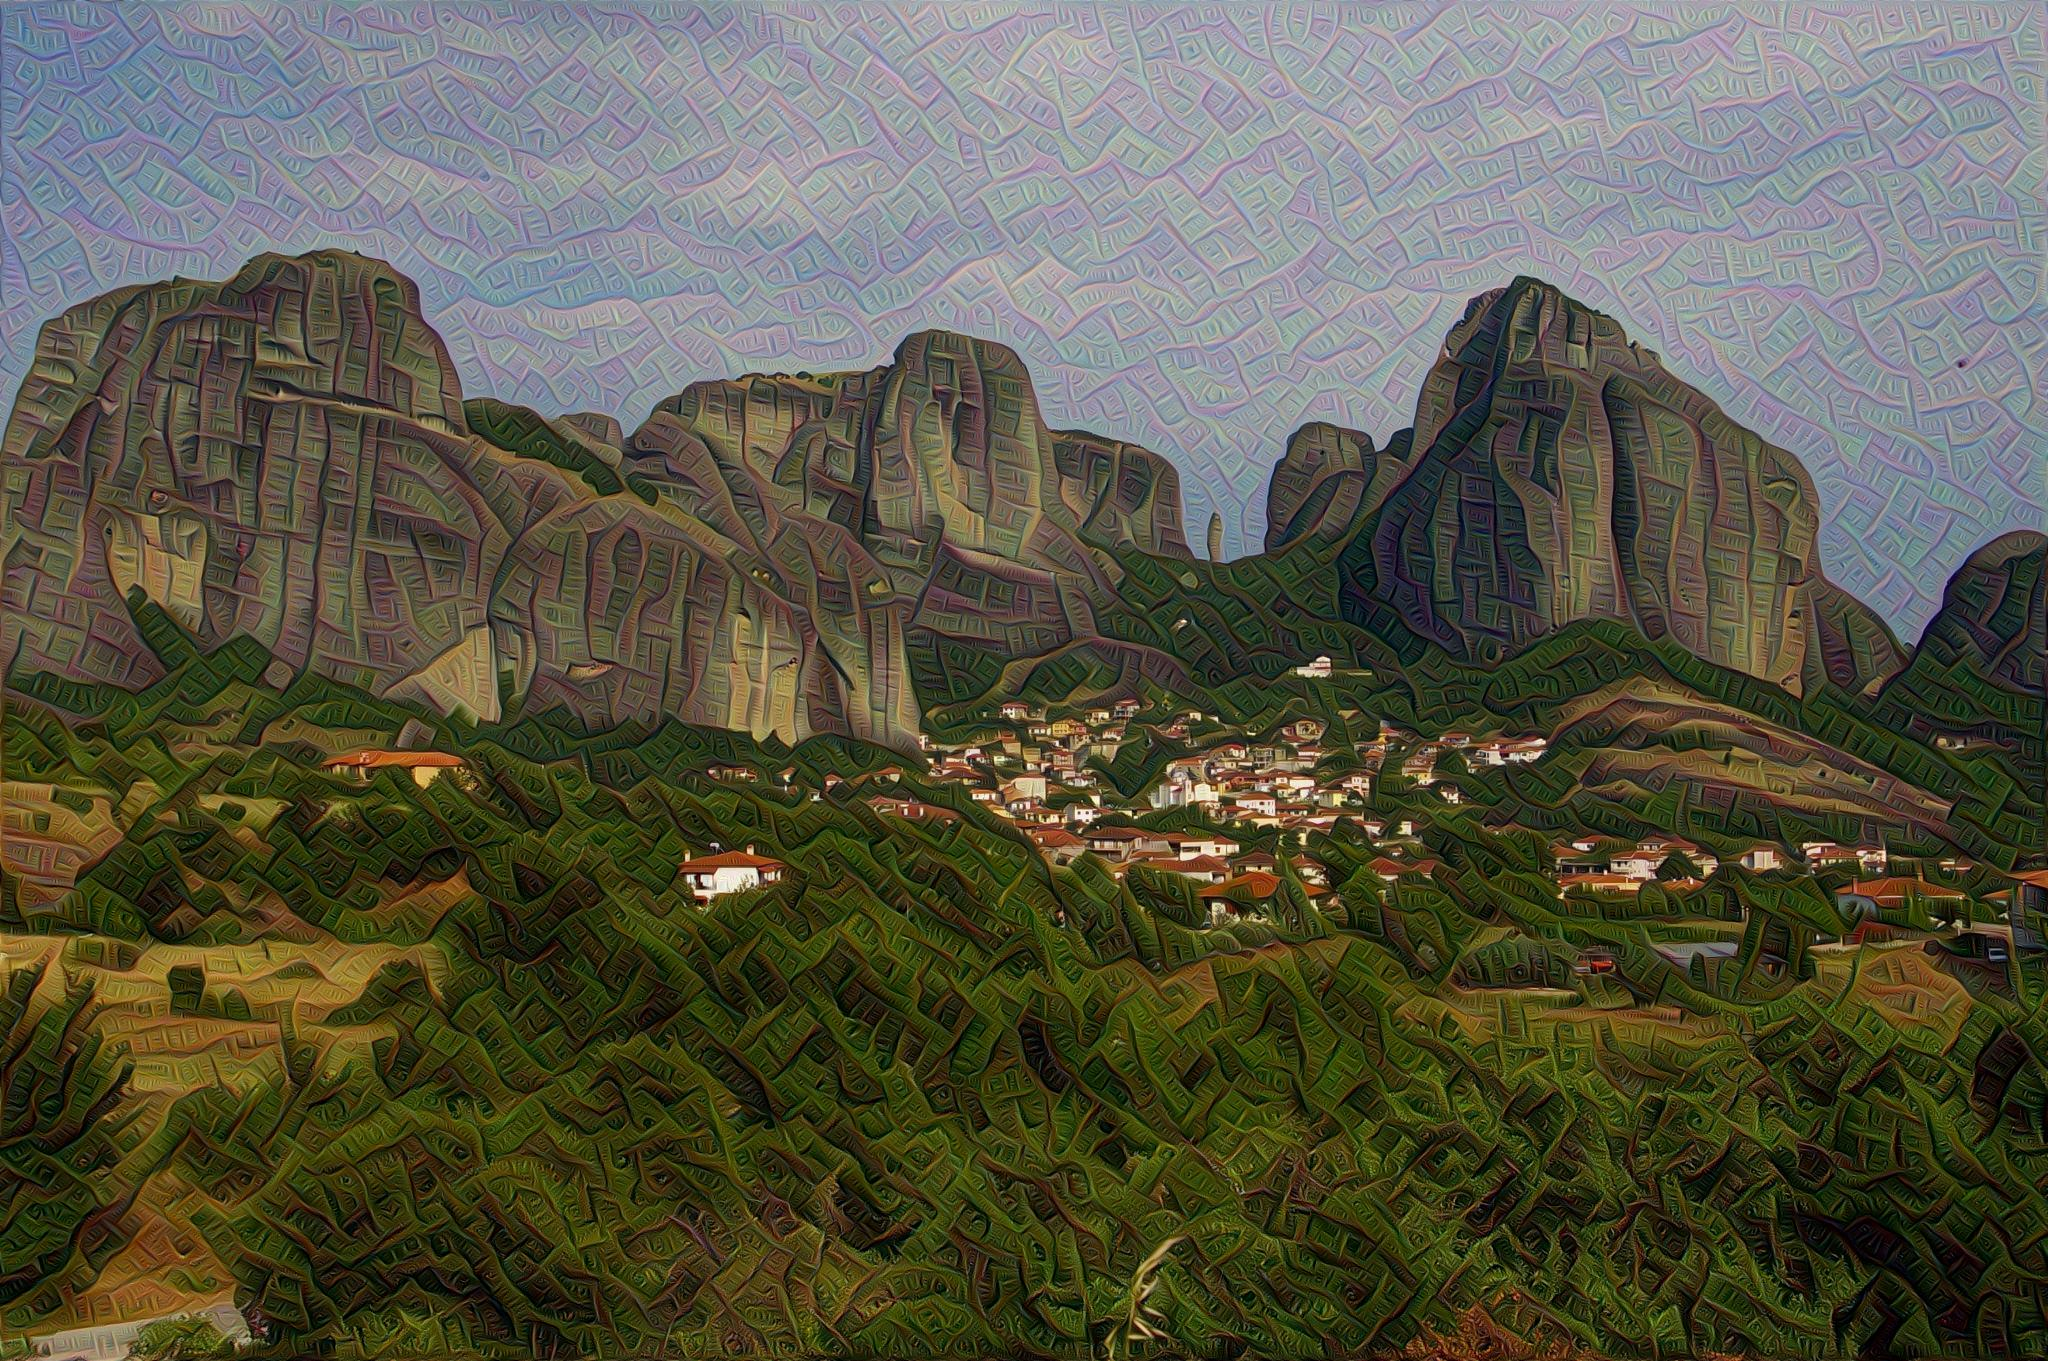
\includegraphics[width=0.7\linewidth]{img/applied_neuron.jpg}
	\caption{A \textit{Deep Dream} onto a landscape which maximizes the activation of the top neuron from figure \ref{fig:neuronreact}.\cite{imgmeteora}}
	\label{fig:applieddream}
\end{figure}

% https://research.googleblog.com/2015/06/inceptionism-going-deeper-into-neural.html



\subsection{TODO: Mathematical Aspects}
Similar to the training process of a network, the dreaming algorithm is an optimization problem.
But rather than training a network to classify samples, one takes a pretrained network and modifies the input so that some neurons in the net get more activated.


When looking at the training process of a (convolutional) neural network, one can see that the weights and biases are changed so that a given error function is minimized.
Because the error function, for instance \emph{mean squared error}, has a lot of dependencies to the weights and biases the derivation is very complex if not even infeasible.
That's why the \emph{gradient descent} algorithm is used to find the (global) minimum of the function\footnote{however, using the gradient descent often solely leads to a local minimum} by taking small steps into the direction of the minimum.
The partial derivative $\frac{\partial C}{\partial w}$ in respect to the weights $w$ and $\frac{\partial C}{\partial b}$ to the biases $b$ of the cost function C is used to calculate how quickly the cost changes when the weights and biases are changed.

So in order to learn a network there are two essential steps:
First there is the \emph{forward} pass, where a sample gets classified by the net.
Afterwards the error made by the network is calculated with the given cost function.
The second step, the \emph{backward} pass, consists of the algorithm of the \emph{gradient descent}, often called \emph{backpropagation} in the context of neural networks.
Based on the error, also called \emph{loss}, the gradients for every weight and bias are calculated.

The negative gradients can be interpret as the direction in which the function should step in order to minimize the loss.
For the weight adjustment we merely add the gradients to the weights and biases.
To prevent too slow learning or \enquote{overshooting} a local minimum a \emph{learning rate} is introduced which is multiplied with the gradients.

As already mentioned in the introduction of this section, the goal of the \emph{Deep Dream} algorithm is not to minimize the cost function, but to modify the input so that the activations of certain neurons are maximized.
For example one can choose a whole layer within the net or just some neurons of a layer whose outputs should be maximized according to the L2 norm.
A normal forward pass up until the specified layer will compute the activation values.
The backward pass requires the gradients of the specified layer to be set.
This can be done in several ways, at this point just assume that the gradients are set to the same values as the activation values of that layer.
By starting the backward pass the backpropagation algorithm composes the gradient of each previous layer to compute the gradient of the whole sub model by differentiation using the chain rule.\cite{caffe-backward}
That's why the gradients (or at least the values) of the specified layer has to be set to something, because every layer needs the gradients from its previous layer in order to work.


When the backward pass is done, all gradients are computed.
Obviously the gradients consists of as many values as there are weights and biases.
But with Deep Dream only the weights of the input layer are important, because these can be added to the input image.
By adding the gradients, the activation values at the specified layer will increase or decrease and with that, respectively the features will become more or less present.

\subsection{Optimizations}
\label{sec:optimizations}
Just like in a normal training process of a network, \emph{Deep Dream} is done with multiple iterations.
By repeating the process over and over again, the features become more and more present up to a certain extent.

Another thing that is commonly used is a \emph{step size}, also called \emph{learning rate} in neural networks.
Instead of just adding the gradients as they are, one can increase or decrease the effect by choosing a $step size < 1$ and $> 1$ respectively.

Aside from these two rather simple techniques, \emph{octaves} were also introduced.
The purpose of this procedure is to scale the image after every dream step.
An octave refers to one scaled version of the source image.
The increase in image size is supposed to find new features and enhance them.
One starts with the smallest octave and applies the dreaming.
By calculating the difference between the original and the dreamed image the added or removed features are extracted.
For the next octave both the source image and the features of the previous octave get scaled by a scaling factor and are then added up together.
With this technique it is possible to create very large images, which continuously adds more features as the process proceeds.

 
Another small tweak is to use a jitter, that shifts the image along the x and y-axis in a random interval before the forward and backward pass.
This influences the activation values which in turn changes the gradients and hence results in a different image modification.
This jitter shift is undone, after the image is modified.
This small trick does not just lead to different results, it also provides smooth transitions between remarkable enhanced features.

Because enhanced features can look harsh, especially with a high step size, a good way to smooth things out is to use a filter. 
The filter can either be applied after every iteration or after every octave.
In section \ref{sec:evaluation} the best results are presented and the used filters mentioned.
 %TODO eyes bsp


\subsection{Guided Dreaming}
\label{guided-dreaming}
As explained in section \ref{sec:visual-aspects}, instead of increasing the occurrence of present features within an image one can also use a reference image in order to achieve \emph{Guided Dreaming}.
The approach begins with a normal forward pass using the \emph{guide image} and saving the activations at the specified layer.
During the dreaming these activations are set to the gradients at the specified layers.
Doing this leads to results, where the features of the \emph{guide image} are enhanced in the source image.


There are different approaches to guide a dream.
For instance instead of just modifying the input image according to the activations of the reference image, one could also select the best matching correspondences from the guide and the base image.
To achieve this, the dot-products between the saved and the current activations of the image are calculated and then the maxima are used to select the best matches.
This prevents the enhancement of  features in the original image, that aren't there at all.\footnote{cite: https://github.com/google/deepdream/blob/master/dream.ipynb}


